\chapter[Inter- and Intramolecular Interactions in the Solid State]{Inter- and Intramolecular Interactions in the Solid State}
\label{chapter: Inter}
\begin{figure}[H]
\centering
  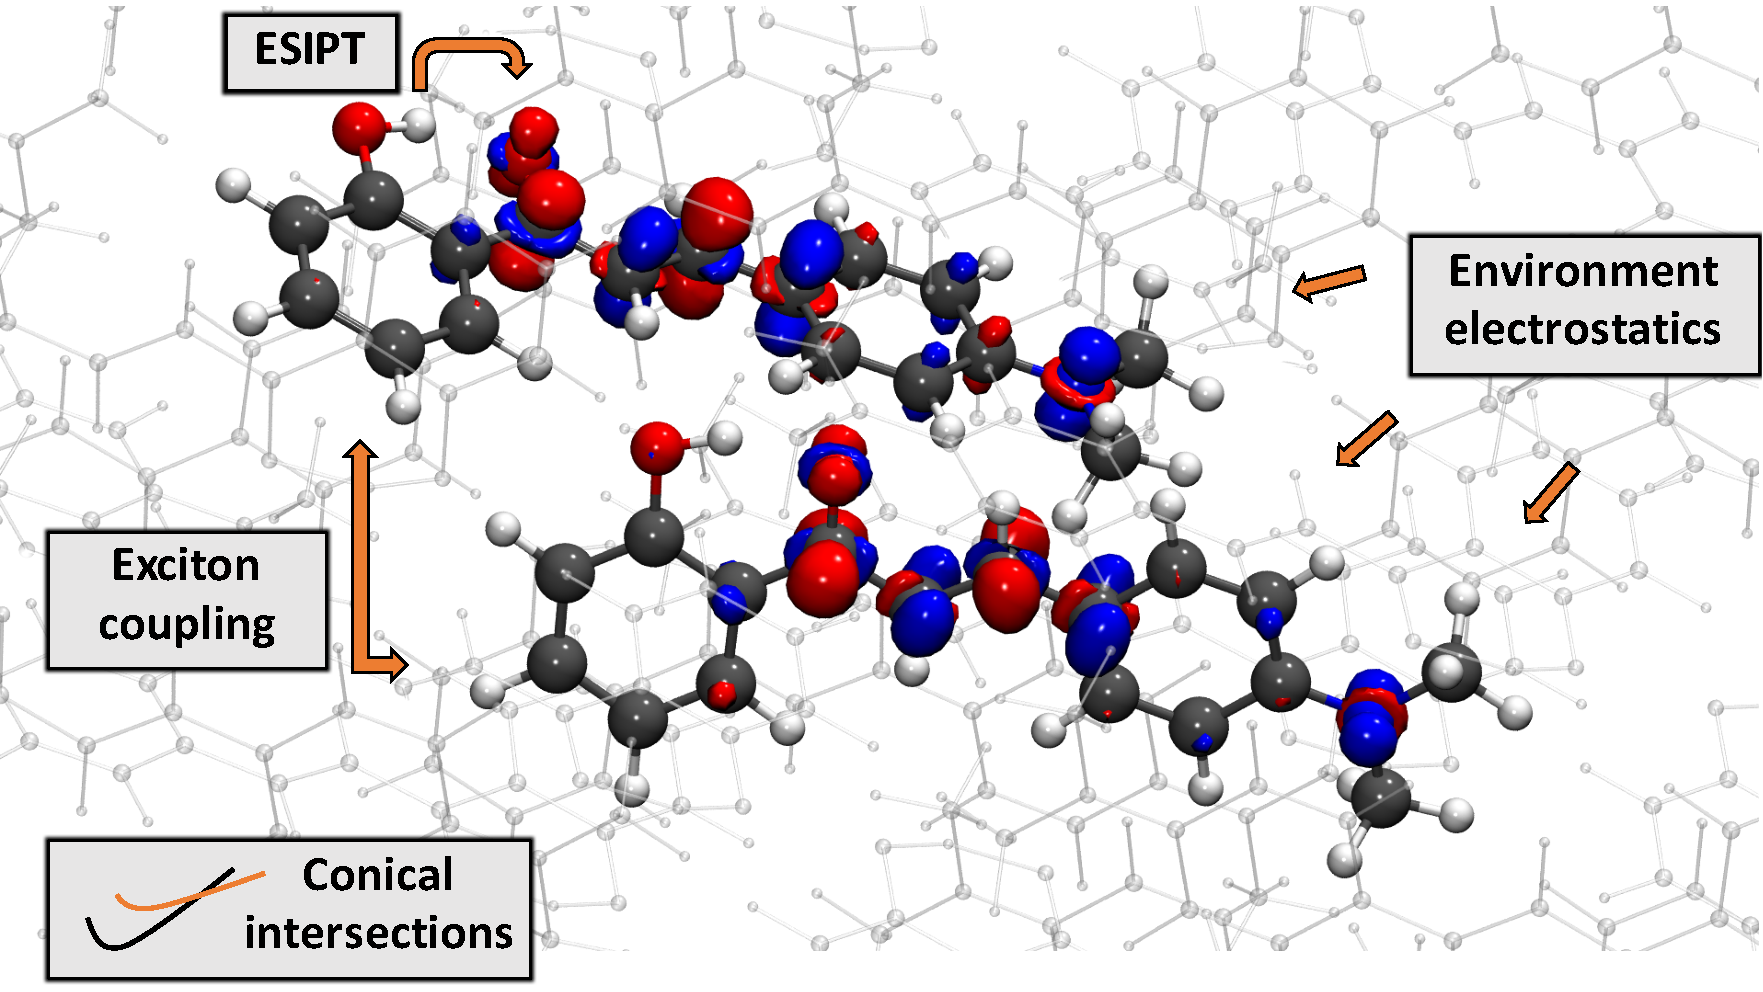
\includegraphics[width=0.6\linewidth]{4IntraInterInteractions/2toc.pdf}
\end{figure}
\section{Introduction}\label{section: Inter_Introduction}
In Chapter \ref{chapter:NRdecay}, the nonradiative decay mechanisms in vacuum were established for the \ac{HC} derivatives \textbf{1}-\textbf{5} (Figure \ref{figure: HC_experimental}). The two extreme cases were compounds \textbf{1} and \textbf{5}, where the methoxy group of \textbf{5} alters the electronic structure of the chromophore. This results in a slight red shift in the absorption, but a more pronounced effect on the relaxation mechanism. Whilst for compound \textbf{1} relaxation through the enol and keto channels is evenly distributed, ESIPT is greatly preferred in compound \textbf{5} due to the increased acidity of the migrating proton. All systems can relax to the ground state \textit{via} an accessible conical intersection in either the enol or keto channel.

In the solid state, compounds \textbf{1}-\textbf{3} undergo \ac{AIE} whereas \textbf{4} and \textbf{5} remain dark. In this chapter, a combination of theoretical models are used to understand the emission properties in the solid state. In particular, we focus how inter- and intramolecular processes determine the emissive properties in the crystal environment. To provide a complete picture of the factors affecting decay mechanisms in these materials, we use a combination of solid state and excited state embedding calculations to systematically account for the different intermolecular interactions present in the molecular crystal. This involves creating cluster models where a central chromophore is treated with a QM electronic structure method and the exterior molecules are described with an \ac{MM} forcefield, in the QM:MM ONIOM approach. As for our nonadiabatic dynamics simulations in Section \ref{section: NRdecay_Dynamics}, in this chapter the two extreme compounds, \textbf{1} and \textbf{5}, shall be used as exemplar systems (Figure \ref{figure: HC_Dimer_Schematic}). In \textbf{1}, chromophores aggregate in a slip-stacking, herringbone structure in an edge to face arrangement. Conversely, in \textbf{5} the dominant motif is the face to face $\pi$-$\pi$ stacking of chromophores.

The work herein was published in reference \citenum{Dommett2017b}. The data shall be presented in dedicated sections here, incorporating the Supporting Information, rather than the letter format chosen for publication, although the order of the discussion remains similar. Important to note that while in ref. \citenum{Dommett2017b} the compounds were labelled as \textbf{1} and \textbf{2}, in this work the original numbering of Chapter \ref{chapter:NRdecay} is retained - thus compound \textbf{2} of ref. \citenum{Dommett2017b} is compound \textbf{5} herein. This chapter is organised in the following way. First, the computational methodology is discussed, where we detail the combination of electronic structure methods and embedding models. Second, since the electronic structure method is \ac{TDDFT} for this section, we benchmark vacuum-phase results against those in Chapter \ref{chapter:NRdecay}. Next, the absorption in the solid state is analysed taking into account monomer and dimer chromophores and the excitonic interactions present in the molecular crystal. Excited state minima and conical intersections are then optimised to determine the excited state relaxation mechanism in the molecular crystal and rationalise the observed fluorescence of \textbf{1} and the nonradiative decay of \textbf{5}. Finally, the results are summarised to offer some design rules for ESIPT/AIE systems. All calculations and analyses were performed by myself apart from the Ewald embedding calculations, implemented and performed by Miguel Rivera. All figures are reprinted with permission from ref. \citenum{Dommett2017b}. Copyright 2018 American Chemical Society.
%%%%%%%%%%%%%%%%%%%%%%%%%%%%%%
\section{Computational Methodology}\label{section: Inter_Computional}
%%%%%%%%%%%%%%%%%%%%%%%%%%%%%%
\begin{figure}[t]
\centering
  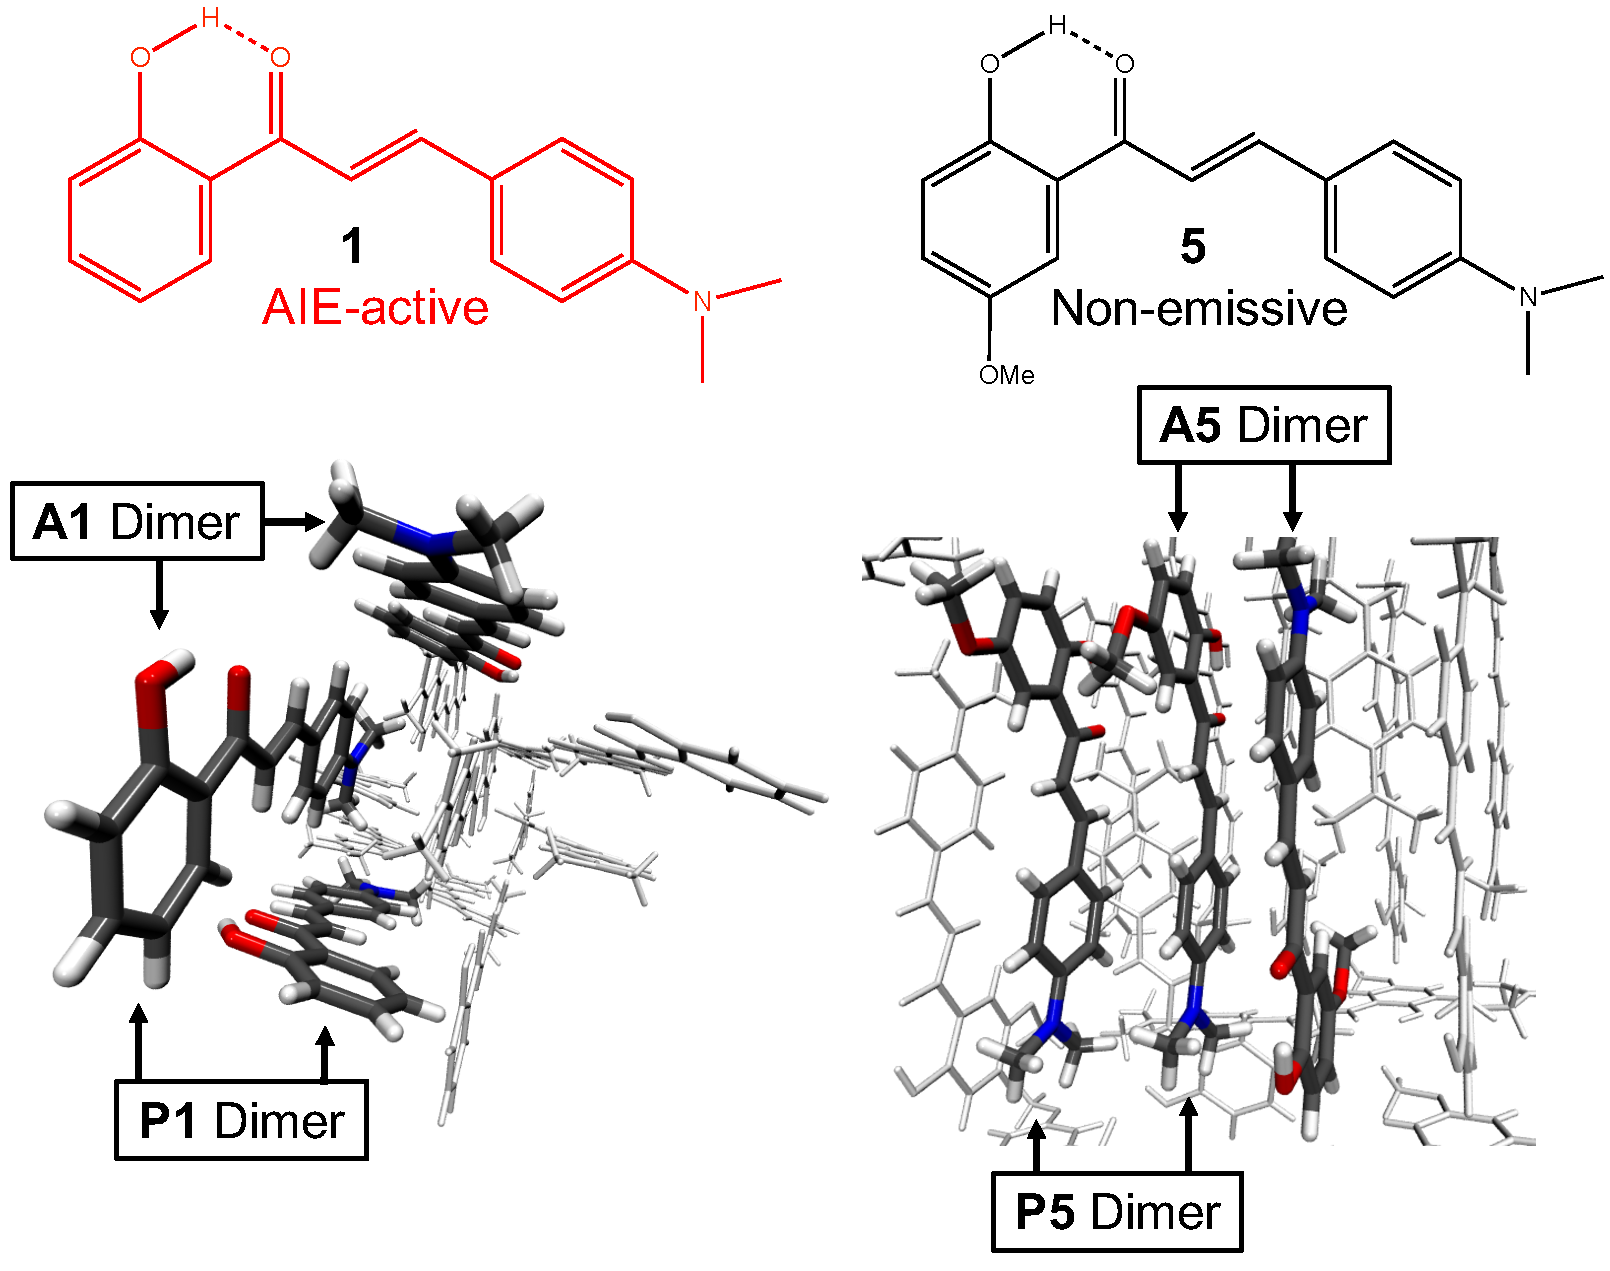
\includegraphics[width=0.9\linewidth]{4IntraInterInteractions/2HC_Schematic.pdf}
  \caption[Molecular, dimer, and crystal structures of \textbf{1} and \textbf{5}]{The molecular and crystal structures of the \textbf{1} and \textbf{5} Compound \textbf{1}, left, displays AIE behaviour, whereas \textbf{5}, right, is nonemissive in both aqueous and solid phases. Also labelled are the parallel (\textbf{P}) and antiparallel (\textbf{A)} dimer configurations.}
  \label{figure: HC_Dimer_Schematic}
\end{figure}
The cluster models of \textbf{1} and \textbf{5} are based on the experimental crystal structures deposited with the CCDC, codes 941991 and 1061608 respectively.\cite{Cheng2015} The crystal structures of \textbf{1} and \textbf{5} were initially optimised using Quantum Espresso in the periodic DFT framework.\cite{QE-2009} Optimisation of each unit cell was carried out with DFT-D2 (PBE) with a plane-wave cutoff of 30 Ry and a Monkhorst-Pack k-point grid of 2x3x2 in accordance with the shape of the unit cell. Clusters of varying size were cut from the DFT-D2-optimised cell for the ONIOM calculations.

The solid state photochemistry of \textbf{1} and \textbf{5} is modelled by applying the ONIOM scheme in a QM:MM protocol using \ac{DFT} and \ac{TDDFT} as the QM electronic structure method.\cite{Byun1999,Frisch2003,Chung2015a} This is an attractive route to efficiently evaluate the mechanism of \ac{AIE}, as the chromophore can be treated within the necessary QM framework whilst the surrounding crystal structure can be evaluated using \ac{MM} methods. For each cluster, the surrounding molecules were fixed in their lattice positions during geometry optimisation of the central chromophore and computed with the AMBER forcefield using ESP charges derived from a vacuum HF/3-21G\textsuperscript{*} calculation of a monomer cut from the crystal structure, allowing electrostatic embedding of a QM-derived electronic density - a scheme we denote AMBER(HF).\cite{Cornell1995}

For all models discussed in the following sections, the focus is four important regions of the \ac{PES}; the Franck-Condon point (FC), enol (\Estar) and keto (\Kstar) minima, and the S\textsubscript{1}/\szero{} MECI. These were established as important points in the vacuum calculations of Chapter \ref{chapter:NRdecay}. Ground and excited state minima and the MECI structures were calculated at the ONIOM($\omega$B97X-D/6-31G(d)):AMBER(HF) level within the DFT and TD-DFT framework. Energies at the ground and excited state minima were recalculated  with the 6-311++G(d,p) basis set. Additionally, RI-CC2/def2-TZVP embedded calculations were performed. The CIOpt algorithm of Levine, Coe and Martinez was again applied to determine the location of the minimal energy conical intersection (MECI) structures.\cite{Levine2008} The nature of the MECIs were confirmed with the CASSCF method in both vacuum and solid state, explained in detail below.

For each of \textbf{1} and \textbf{5}, three ONIOM((TD-)DFT):AMBER(HF) clusters of differing size are evaluated:
\begin{itemize}
    \item \textbf{M7}: all molecules within 7{\AA} of a central monomer chromophore
    \item \textbf{M15}: all molecules 15{\AA} from the central monomer
    \item \textbf{D7}: all molecules within a 7{\AA}-radius from the centroid of a dimer chromophore
\end{itemize}
The cluster models are visualised in Figures \ref{figure: HC_Cluster_Models}-\ref{figure: HC_Dimer_Models}. Two \textbf{D7} dimer models were considered due to the prominence of two dimer arrangements in each of the crystal structure, where monomers are arranged parallel (\textbf{P}) and antiparallel (\textbf{A}). The parallel stacked dimer model is denoted \textbf{D7-P} and the antiparallel configuration is \textbf{D7-A}. These stacking arrangements are shown in Figure \ref{figure: HC_Dimer_Schematic}.

\begin{figure}
\centering
  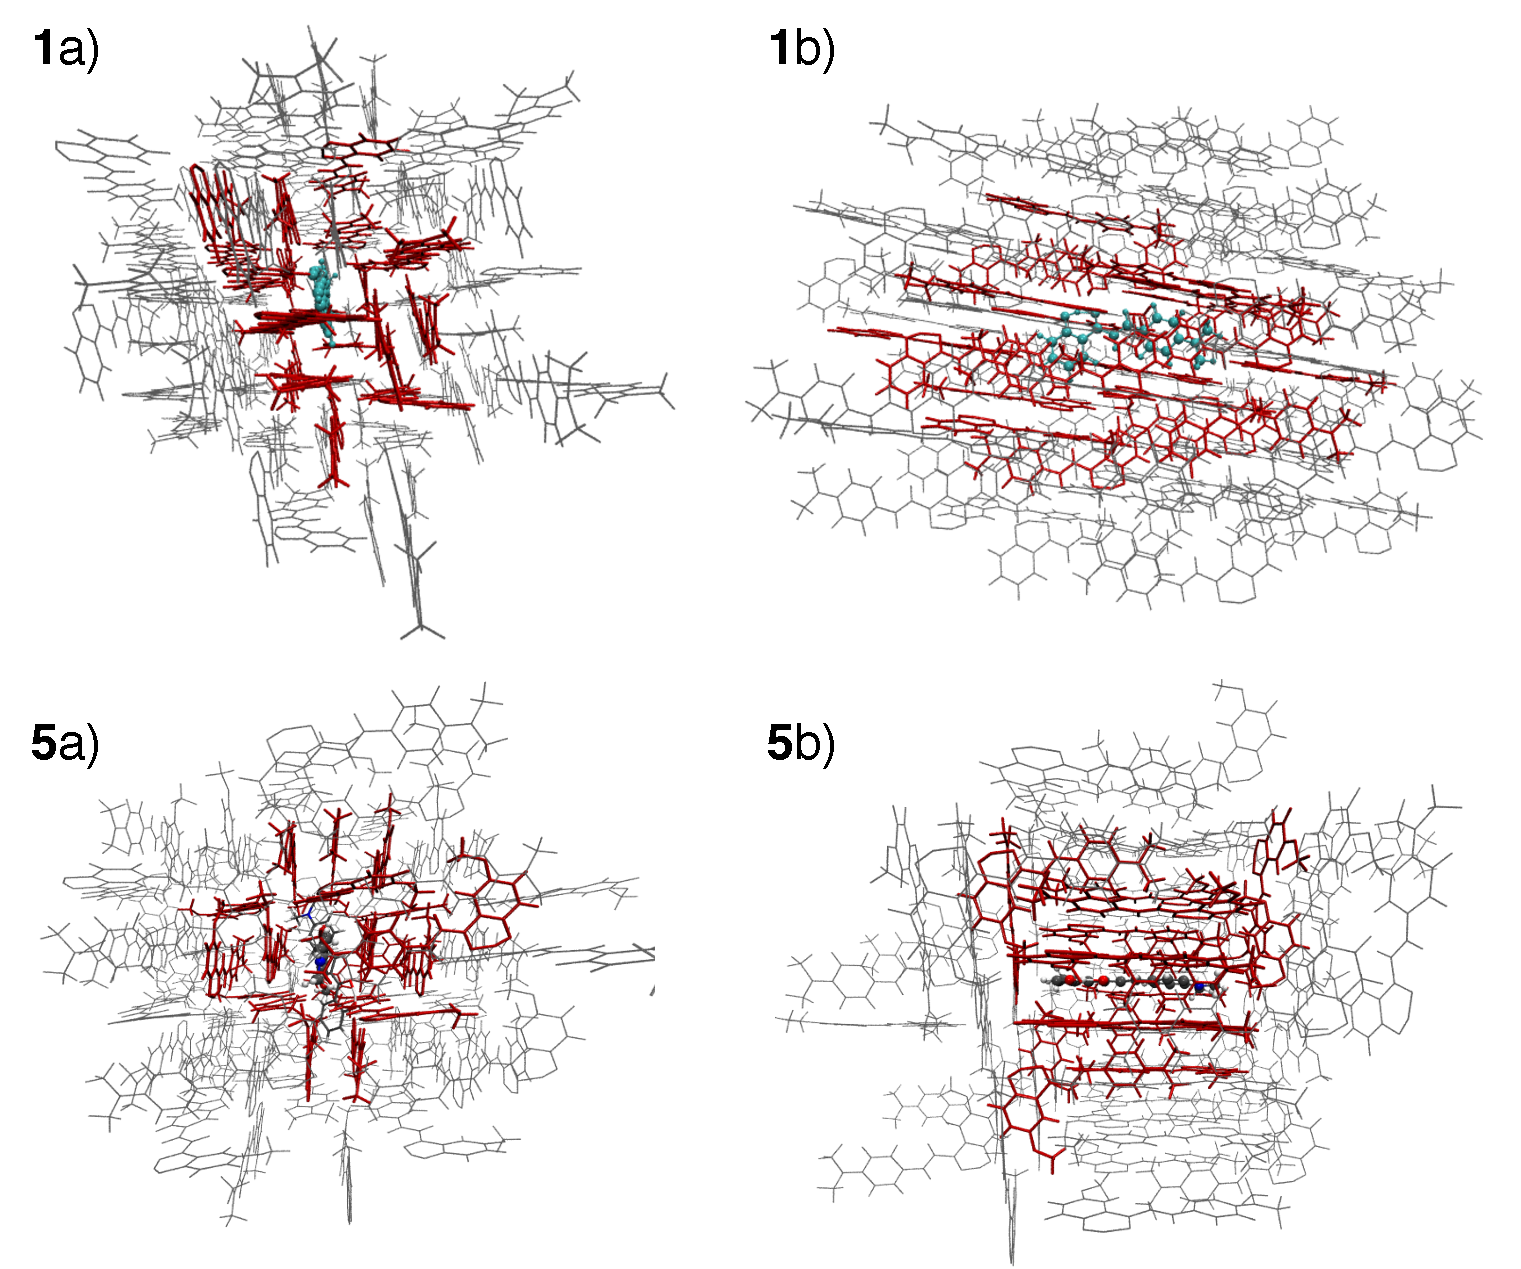
\includegraphics[width=0.8\linewidth]{4IntraInterInteractions/HC_Cluster_Models.pdf}
  \caption[The \textbf{M7} and \textbf{M15} cluster models]{Two viewpoints \textit{a} and \textit{b} of the \textbf{M7} and \textbf{M15} models for compounds \textbf{1} and \textbf{5}. The central molecule is shown in cyan, surrounded by an increasing radius of 7{\AA} (red, \textbf{M7}) and 15{\AA} (red+grey, \textbf{M15}).}
  \label{figure: HC_Cluster_Models}
\end{figure}

\begin{figure}
\centering
  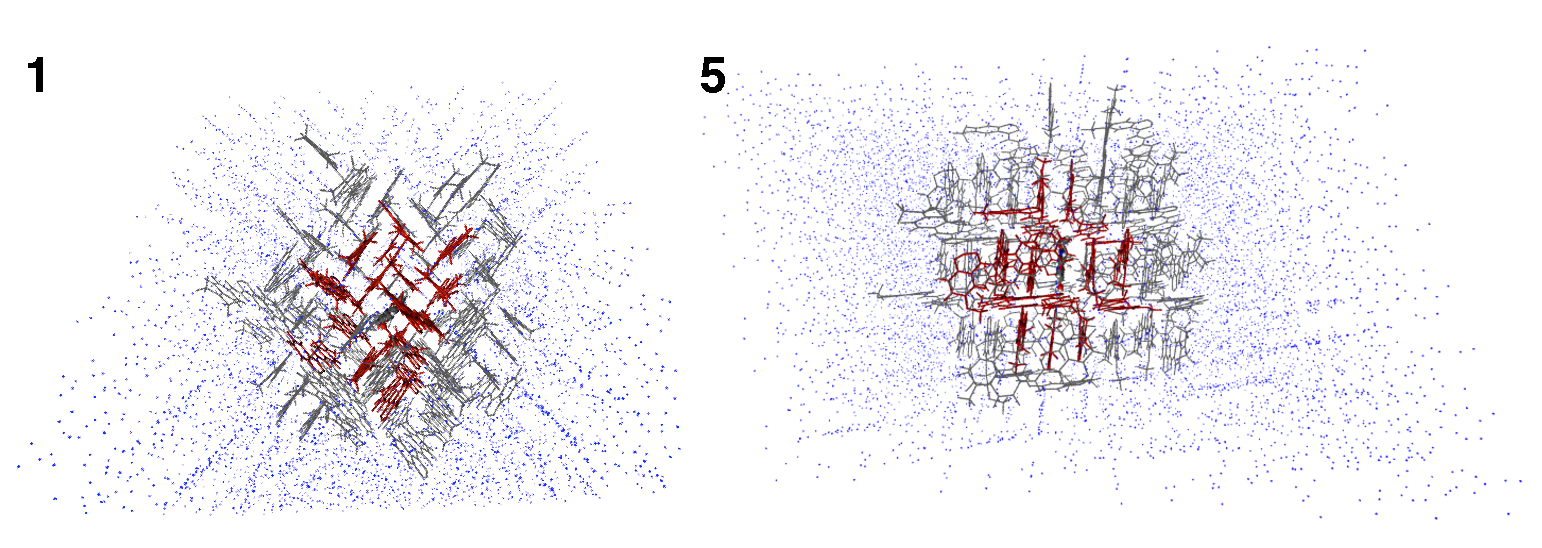
\includegraphics[width=0.9\linewidth]{4IntraInterInteractions/HC_Ewald.pdf}
  \caption[The \textbf{Ewald} charges of \textbf{M15}]{Visualisation of the \textbf{Ewald} model for compounds \textbf{1} and \textbf{5}, where the \textbf{M15} model (cyan + red + grey) is embedded in Ewald point charges, shown in blue.}
  \label{figure: HC_Ewald}
\end{figure}

\begin{figure}
\centering
  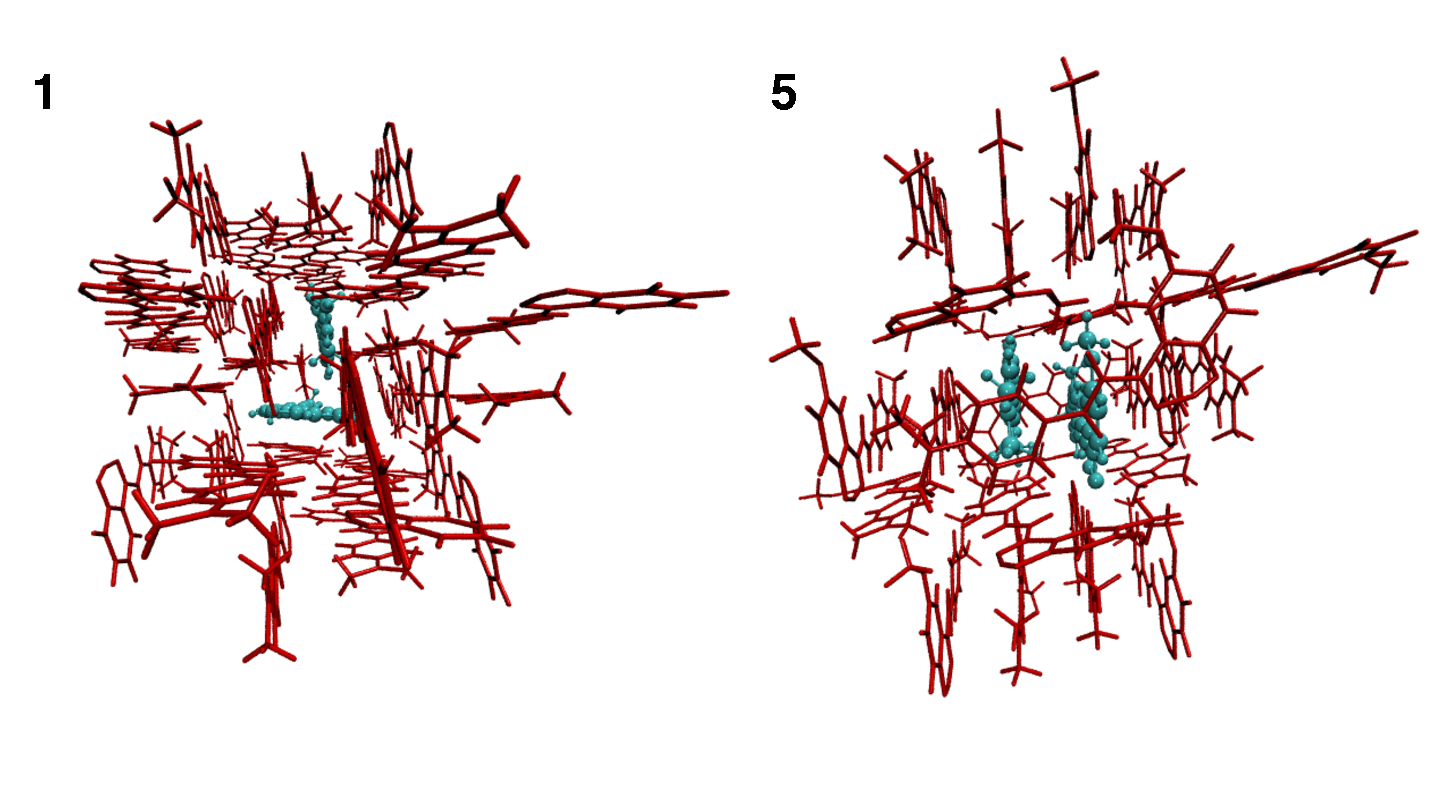
\includegraphics[width=0.9\linewidth]{4IntraInterInteractions/HC_Dimer_Models.pdf}
  \caption[The \textbf{D7} cluster models]{The \textbf{D7} model for compounds \textbf{1} and \textbf{5}. The dimer chromophore is shown in cyan, and the surrounding molecules within a radius of 7{\AA} are shown in red.}
  \label{figure: HC_Dimer_Models}
\end{figure}

ONIOM calculations were performed with the electrostatic embedding scheme. Post optimisation, single point calculations in vacuum of each ONIOM((TD-)DFT:AMBER(HF) geometry were performed to evaluate how the environment influences the energy. To assess the role of the electrostatic potential during relaxation, we also perform optimisation for the \textbf{M7} and \textbf{M15} models with mechanical embedding. The nature of vertical excitations in solid state was assessed using the CALCDEN method, which classifies electronic excitations based on the electronic density localisation between donating and accepting orbitals.\cite{Crespo-Otero2012,Sen2013} 

To simulate the long-range periodic electrostatic environment experienced by the chormophore, the \textbf{M15} model was embedded in point charges derived from the Ewald method of Derenzo, Klintenberg and Weber, as described in Section \ref{section: excited_states_crystals}.\cite{Klintenberg2000,Derenzo2000} In the \textbf{Ewald} model, the chromophore was embedded in a set of point charges for each of the \szero{} and \sone{} minima and MECI geometries found with \textbf{M15} model. The initial charges were the same ESP charges used in the ONIOM models. 500 points had a fixed charge value, 1000 sample sites were used and the supercell was comprised of 4x4x4 unit cells.

The topology of the PES between the \Kstar{} minimum and the MECI was explored for the \textbf{M15} model through \ac{LIIC}, using the 6-31G(d) basis set. A relaxed geometry scan of the torsional angle $\theta$\textsubscript{tor} was also performed for the \textbf{M15} model with the 6-31G(d) basis set to probe the \ac{PES} of the \Kstar{} state. All ONIOM calculations were performed with Gaussian 09 (rev D.01).\cite{g09}

The energies at the FC state and \Kstar{} minimum for the \textbf{M15} chromophore were calculated at the RI-CC2/def2-TZVP level of theory using point charge embedding with TURBOMOLE v7.0.\cite{Hattig2002,Turbomole} The point charges were located at the atomic positions of the MM-atoms in the \textbf{M15} model.

We validate the TDDFT calculated MECI geometry of \textbf{1} and \textbf{2} in the solid state by optimising the conical intersection with the state-averaged complete active space self-consistent field  method, using an active space of 12 electrons in 11 orbitals with the 6-31G(d) basis set (SA-CASSCF(12,11)/6-31G(d)):AMBER(HF). The MECI geometry is optimised within the \textbf{M7} model with AMBER forcefield to describe the MM-level, in which all the positions of all MM atoms are frozen during the optimisation. All CASSCF calculations were performed using the MOLCAS@UU v8.0 binaries, using  the Tinker v.6.3.3 interface for the QM/MM calculations. 

Further understanding can be achieved by calculating the excitonic couplings for the relevant dimers. The diabatization scheme of Troisi was implemented to calculate the excitonic couplings $J$.\cite{Arago2015} This scheme incorporates both the short-range (exchange, orbital overlap, charge-transfer) and long-range Coulomb interactions. 

The multi-model approach ensures size-consistency of the MM-region, evaluates the role of short and long-range interactions, explicitly models the long-range electrostatic potential from the crystal, and determines the role of excitonic coupling on the mechanistic interpretation.
%%%%%%%%%%%%%%
%%%%%%%%%%%%%%
\section{Results}\label{section: Inter_Results}
\subsection{Benchmarking of TDDFT}\label{section: Inter_benchmark}
Since the electronic structure method of choice in this chapter is \ac{TDDFT}, it is important to initially benchmark against the post-Hartree Fock methods used in Chapter \ref{chapter:NRdecay}. In this section we briefly compare the vertical excitations, relaxation pathways, and conical intersection geometries. Previous studies have shown that TDDFT performs well compared to CC2 for studying ESIPT.\cite{Aquino2005}

For the vertical excitations in vacuum with TD-$\omega$BX-D/6-311++G(d,p) (Table \ref{table: solid_vertical excitations}), the results of \textbf{1} and \textbf{5} compare well with CC2/def2-TZVP (Table \ref{table: HC_VEs}). The character of the first three states is the same across the  methods, with \sone{} as the bright state \pipistar{} for \textbf{1}. For compound \textbf{5}, with TDDFT \stwo{} borrows intensity from \sone{}, as with CC2 and ADC(2). The relative red shift of \textbf{5} is also similar (0.17 with CC2, 0.12 with TDDFT). It is evident that at the Franck-Condon geometry TDDFT can provide the same trends as CC2 and ADC(2), but at lower computational cost.

The excited state minima and \ac{MECI}s in the enol and keto channels were also optimised for \textbf{1}-\textbf{5} in vacuum with TD-$\omega$BX-D/6-311++G(d,p). The energies are shown in Figure \ref{figure: HC_TDDFT_Vac}. For \textbf{1} and \textbf{5}, the surfaces were also obtained at TD-$\omega$BX-D/6-31G(d) level, shown in Appendix B. The energies obtained are very similar to ADC(2) and CC2, with the keto minima at lower energy than the enol minima for \textbf{1}-\textbf{3}. As with ADC(2) and CC2, no enol minima were obtained with TDDFT, and thus the same propensity for ESIPT will be witnessed for \textbf{5}. The enol minima occur at more planar $\theta_{tor}$ angles for \textbf{1}-\textbf{3}, and therefore a larger emission energy is predicted. For \textbf{5}, similar is seen with the keto minimum, where the equilibrium geometry is more planar and thus a larger energy gap is present.

For the \ac{MECI}s in vacuum, the geometry obtained with TDDFT compare well with those obtained with CASSCF and CC2. Indeed, the TDDFT geometry is most similar to CASSCF and does not suffer from the problems of ADC(2). The \Kstar{} MECI in vacuum was calculated for \textbf{1} and \textbf{5} with the SA(2)-CASSCF(12,11)/6-31G(d). The geometries are compared to those obtained in vacuum at the {\highlevel} level of theory in Figure \ref{figure: MECI_TDDFT_vs_CASSCF_VAC}. There is an excellent agreement between the CASSCF(12,11)/6-31G(d) calculated MECI geometry (shown in cyan) and the {\highlevel} geometry (black). For compound \textbf{1}, left, the RMSD between the two methods is 0.11 \AA. For compound \textbf{5}, the geometries are more deviated, with an RSMD of 0.59 \AA. This deviation arises due to the dihedral angle at the amino group of the molecule, which is 13{\textdegree} for TDDFT and 60{\textdegree} for CASSCF. The dihedral angles of the deprotonated phenol ring, the coordinate which drives the convergence of states, are a good match (89.9{\textdegree} for TDDFT vs 90.2{\textdegree} for CASSCF). The agreement between the TDDFT \Kstar{} conical intersection with the geometry of the CASSCF-predicted MECI in vacuum show that the protocol we employ to explore the PES with TDDFT is robust. As such the choice of TDDFT should not alter the conclusions obtained with ADC(2) and CC2. In this chapter, we also carry out single point calculations with CC2, but TDDFT is the main method chosen due to its computational efficiency and readily available implementation for QM:MM methods in ONIOM with Gaussian software. The conical intersections are also calculated using the QM:MM scheme incorporated in Molcas, using SA(2)-CASSCF(12,11)/6-31G(d):AMBER(HF) to validate the conical intersections calculated with TDDFT in ONIOM.
\begin{figure}[t]
\centering
  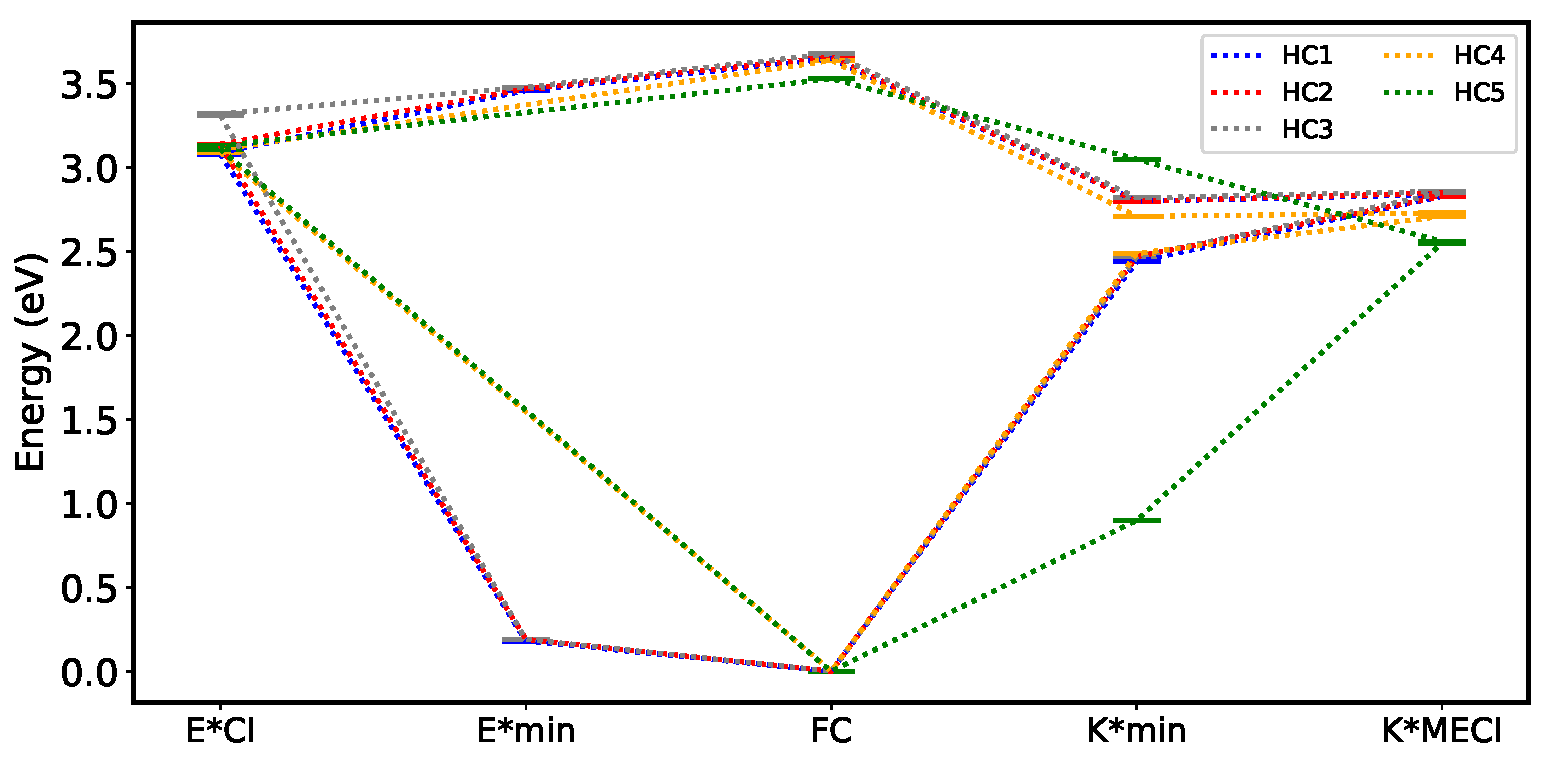
\includegraphics[width=0.8\linewidth]{4IntraInterInteractions/2HC_energies_vac_TDDFT.pdf}
  \caption[The vacuum PES of \textbf{1}-\textbf{5} with TDDFT]{The critical points on the \ac{PES} for \textbf{1}-\textbf{5} obtained at (TD-)$\omega$BX-D/6-311++G(d,p) in vacuum.}
  \label{figure: HC_TDDFT_Vac}
\end{figure}

\begin{figure}
\centering
  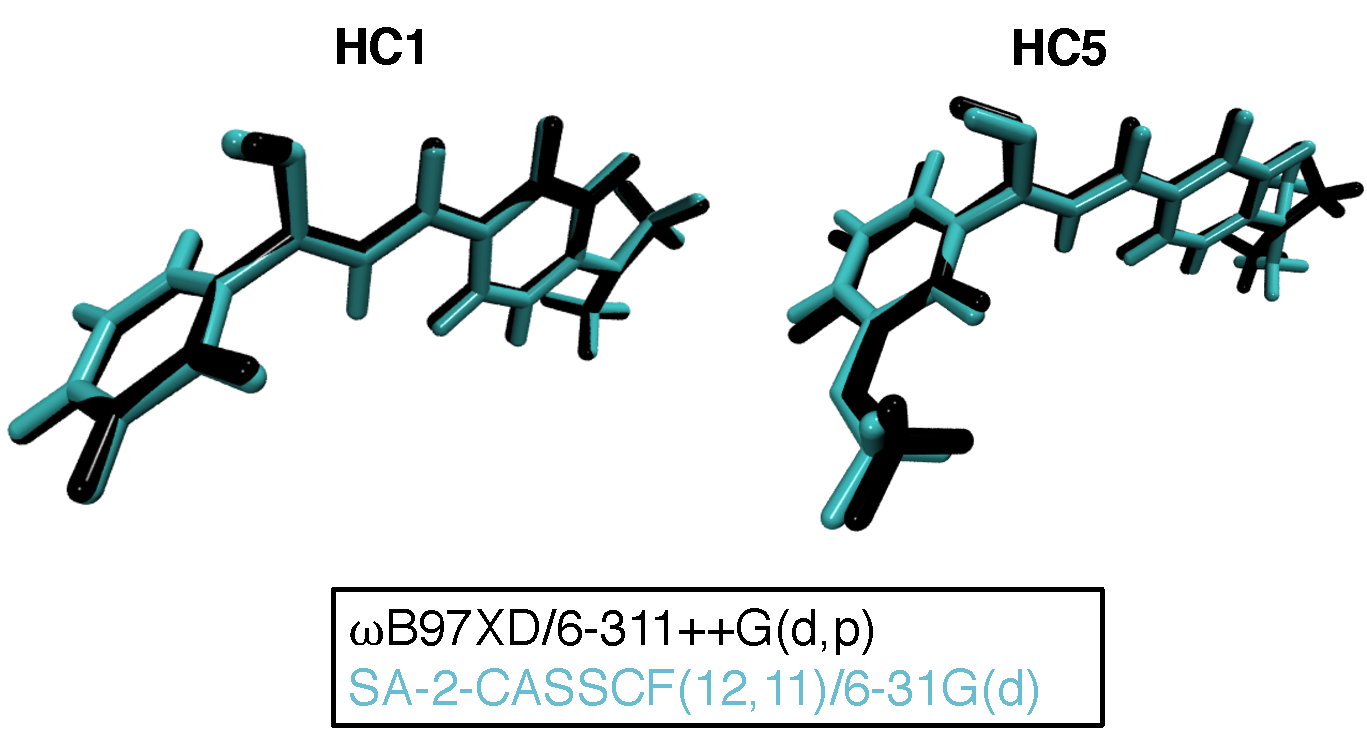
\includegraphics[width=0.75\linewidth]{4IntraInterInteractions/MECI_TDDFTvsCASSCF_VAC.pdf}
  \caption[Comparison of MECIs obtained with TDDFT and CASSCF]{Comparison of the \highlevel (black) and SA-CASSCF(12,11)/6-31G(d) (cyan) MECI geometries for compounds \textbf{1} (left) and \textbf{5} (right).}
  \label{figure: MECI_TDDFT_vs_CASSCF_VAC}
\end{figure}

\subsection{Absorption in the Molecular Crystal}\label{section: Inter_absorption}
In this section examine the absorption in the molecular crystal. For all models, the crystal environment shifts the bright state to the red with respect to absorption in vacuum. The bright state calculated for \textbf{1} with the \textbf{M} and \textbf{D} models (Table \ref{table: solid_vertical excitations}) are in very good agreement with the experimental value of 3.3 eV.\cite{Cheng2015} The bright state is calculated as 2.93 eV with RI-CC2/def2-TZVP. In the case of \textbf{5}, where no experimental absorption spectrum has been published, the energies predicted with all models are in the range of 3.4-3.5 eV. In this case the RI-CC2/def2-TZVP value of 3.33 eV aligns better with TDDFT than in \textbf{1}. There is no significant intermolecular charge transfer upon excitation in either material. 

\begin{table}
  \centering
  \caption[Excitation energies in the solid state]{Excitation energies and oscillator strengths for the first three excited singlet states of \textbf{1} and \textbf{5} in various models. Energies calculated at $\omega$B97X-D/6-311++G(d,p) level of theory and given in eV.} 
  \label{table: solid_vertical excitations}
  \begin{tabular}{lccccc}
    \hline
     & &
    \multicolumn{2}{c}{Compound \textbf{1}} 
    &
    \multicolumn{2}{c}{Compound \textbf{5}}\\
    \hline
     & & Energy (eV) & Osc.(\textit{f}) &
    Energy (eV) & Osc.(\textit{f})\\
    \hline
    
    \multirow{3}{*}{\textbf{Vacuum}} & 
	\sone{} & 3.65 & 1.143 & 3.53  & 0.870 \\
    & \stwo{} & 3.95 & 0.007 & 3.87  & 0.244 \\
    & \sthree & 4.16 & 0.002  & 3.93  & 0.013 \\
    \hdashline
   
    \multirow{3}{*}{\textbf{M7}} & 
	\sone{} & 3.20 & 1.177 & 3.42 & 0.905\\
    & \stwo{} & 4.10 & 0.001 & 3.74 & 0.236\\
    & \sthree & 4.27 & 0.030 & 4.00 & 0.002\\
    \hdashline
    
     \multirow{3}{*}{\textbf{M15}} & 
	\sone{} & 3.30 & 1.174 & 3.40 & 1.005\\
    & \stwo{} & 4.07 & 0.002 & 3.72 & 0.147\\
    & \sthree & 4.18 & 0.018 & 4.01 & 0.015\\
    \hdashline
    
    \multirow{3}{*}{\textbf{Ewald}} & 
	\sone{} & 3.30 & 1.192 & 3.50 & 0.815\\
    & \stwo{} & 4.06 & 0.002 & 3.81 & 0.320\\
    & \sthree & 4.16 & 0.015 & 3.90 & 0.008\\
    \hdashline
    
    \multirow{3}{*}{\textbf{D7-P}} & 
	\sone{} & 3.16 & 0.017 & 3.18 & 0.029\\
    & \stwo{} & 3.26 & 2.128 & 3.51 & 1.379\\
    & \sthree & 3.57 & 0.003 & 3.60 & 0.001\\
    \hdashline
    
    \multirow{3}{*}{\textbf{D7-A}} & 
	\sone{} & 3.10 & 0.061  & 3.05 & 0.000 \\
    & \stwo{} & 3.35 & 2.063 & 3.42 & 1.947 \\
    & \sthree & 3.79 & 0.006 & 3.61 & 0.012 \\
    \hline
  \end{tabular}
\end{table}
The electrostatic potential generated by the whole crystal (in the \textbf{Ewald} model) has a negligible effect for the vertical excitations of \textbf{1}, with a convergence of 3.3 eV for the bright state. In the case of \textbf{5}, a more polar structure, the effect is more significant, with a shift in the energy of around 0.1 eV. Since this is in the order of the shift associated with vibrations and does not change the nature of the excited states, even the smaller cluster models (\textbf{M7} and \textbf{D7}) can capture the main electrostatic influence on the photoexcitation.\cite{Crespo-Otero2012} However, more accurate crystalline properties would be achieved by using a more sophisticated apporach for the low-level system rather than molecular mechanics, such as QM:QM' embedding methods currently under development in the Crespo-Otero group. This is particularly important for finding equilibrium structures on the excited state surface.

In going from a monomer chromophore to a dimer chromophore, the bright state shifts from \sone{} to \stwo.  For the Frank-Condon (FC) geometry, the electronic density is delocalised over both molecules in the chromophore. As a consequence of  excitonic coupling, the bright state is blue shifted in 0.06 eV and 0.15 eV  for \textbf{1} and 0.23 eV and 0.32 eV for \textbf{5} (\textbf{M7} model as reference). This is typical of H dimers within the Kasha excitonic coupling model, with oscillator strengths of \stwo{} almost double those of the monomer species in \sone.\cite{Kasha1965a} While the splitting is more significant for \textbf{5}, this does not alone explain the different properties of \textbf{1} and \textbf{5}. 

The largest coupling (Table \ref{table: Inter_Jcoupling}) in each compound occurs when the monomers are aligned antiparallel (\textbf{A}), of the order of 100 meV, which are in the order of those obtained for some organic semiconductors.\cite{Fornari2017} These couplings result from the favourable alignment between the nitrogen of one monomer and carbonyl group on the other monomer (approximately 4.5{\AA}). Recently, the effect of excitonic couplings on the nonradiative constants for AIE was evaluated.\citep{Li2017} For a set of five highly aromatic conjugated molecules, with \textit{J}s in the order of 10 meV, the authors found that excitonic coupling always increases the nonradiative decay constants. Based on these vibronic models, in the \Estar{} form, a larger \textit{J} on the nonradiative vibrational decay should be expected for \textbf{5}. In the next chapter, the excitonic couplings of the \textbf{HC} crystals shall be investigated in more detail.
\begin{table}
\centering
\caption[Exciton coupling in dimers of \textbf{HC1} \& \textbf{5}]{\textit{J} coupling values (eV) between units in dimers of \textbf{1} and \textbf{5} in the \textbf{D7} models}
\label{table: Inter_Jcoupling}
  \begin{tabular}{lcc}
    \hline
     & 
     {Compound \textbf{1}} &
     {Compound \textbf{5}}\\
    \hline
     & \textit{J} (eV)& 
    \textit{J} (eV)\\
    \hline
    {\textbf{D7-P}} &

    0.060 & 0.112\\
    {\textbf{D7-A}}
    & 0.105&0.150\\
    \hline
\end{tabular}
\end{table} 
%%%%%%%%%%%%%%%%%%
%%%%%%%%%%%%%%%%%%
\subsection{Radiative \textit{vs.} NonRadiative Decay}\label{section: Inter_Relaxation}
%%%%%%%%%%%%%%%%%%
%%%%%%%%%%%%%%%%%%
Relaxation to either \Estar{} or \Kstar{} minima will follow photoexcitation. The emission energies and oscillator strengths for each model are collected in Table \ref{table: Inter_emis}. In the case of \textbf{1}, significant reabsorption is expected due to the small Stokes shift for the \Estar{} minimum. This has been recently confirmed experimentally.\cite{Zahid2017} For \textbf{5}, oscillator strengths from \Estar{} are extremely small. In this context, no significant emissive response is expected from the \Estar{} state of either material. For \textbf{1}, relaxation in \Estar{} involves localisation of the electronic density on one molecule, whereas delocalisation is observed for \textbf{5}. In vacuum and the \textbf{M7}/\textbf{15} models, \Estar{} is not stable for \textbf{5}. It is stable in the dimer models due to state mixing where some of the \stwo{} character of the monomer mixes with \sone{}, such that there is less electron density lost from the phenol oxygen in \sone{}. 

\begin{table}[t]
\centering
  \caption[Emission energies in the solid state]{Emission energies and oscillator strengths from the enol and keto minima on the \sone{} PES for various models. Energies reported at \highlevel level of theory and given in eV.}
\label{table: Inter_emis}
  \begin{tabular}{lcccc}
    \hline
    &
    \multicolumn{2}{c}{Compound \textbf{1}} 
    &
    \multicolumn{2}{c}{Compound \textbf{5}}\\
    \hline
     & \Estar{} (\textit{f}) & \Kstar{} (\textit{f}) &
    \Estar{} (\textit{f}) & \Kstar{} (\textit{f})\\
    \hline
    
    {\textbf{M7}} & 
	3.03 (1.207) & 2.67 (1.191) & -  & 2.15 (0.461) \\

    {\textbf{M15}} & 
	3.10 (1.225) & 2.61(0.977) & - & 2.17 (0.490)\\
    
    {\textbf{Ewald}} & 
	3.12 (1.214) & 2.66 (1.052) & -  & 2.18 (0.486)\\

    {\textbf{D7-P}} & 
	3.01 (0.479) & 2.56 (0.725) & 2.45 (0.002) & 2.15 (0.312) \\
    
    {\textbf{D7-A}} & 
	2.96 (0.119) & 2.59 (0.616) & 2.81 (0.000)  & 2.32 (0.388) \\
	\hline
  \end{tabular}
\end{table}

Geometries of the \Estar{} and \Kstar{} minima are planar in the solid state. Since no double proton transfer \Kstar{} minimum was found for \textbf{1},  emission is expected from a localised \Kstar{} state. The experimental emission spectrum for \textbf{1} can be assigned to the \Kstar{} state ranging from 1.5-2.1 eV. The predicted values are blue shifted to 2.7 eV (CC2/def2-TZVP predicts emission at 2.2 eV). The flatness of the \sone{} surface with respect to the dihedral angle suggests that emission from a range of geometries is possible. To investigate this, a relaxed geometry scan was performed at \lowlevel:AMBER(HF) for both \textbf{1} and \textbf{5}, where $\theta_{tor}$ was incrementally increased in the \textbf{M15} model and frozen during relaxation, shown in Figure \ref{figure: HC_Oniom_Scan}. Between 0 and 40{\textdegree}, the \sone{} surface is quite flat, whilst the energy gap between \sone{} and \szero{} states ranges from 2.7 eV (f=0.973) to 2.2 eV (f=0.496). The flatness of the surface, and the high oscillator strengths along the coordinate, suggest that emission from a range of dihedral angles less than 40{\textdegree} is possible, in particular since dihedral rotation energetically favourable relaxation pathway in vacuum. Also important to take into account when considering the emission energies are the limitations of the QM:MM method. All of the exterior atoms are frozen and treated at MM level, without the possibility of any mutual polarisation between the regions. As such, the environment cannot respond to the changes in electronic density of the chromophore, which can be rather large in the case of ESIPT systems. As such, the additional relaxation from mutual charge polarisation is not present here, and the emission energies are somewhat overestimated. The dimer models partially alleviate this by having a polarisable molecular counterpart, and the emission energy is reduced. 

\begin{figure}[t]
\centering
  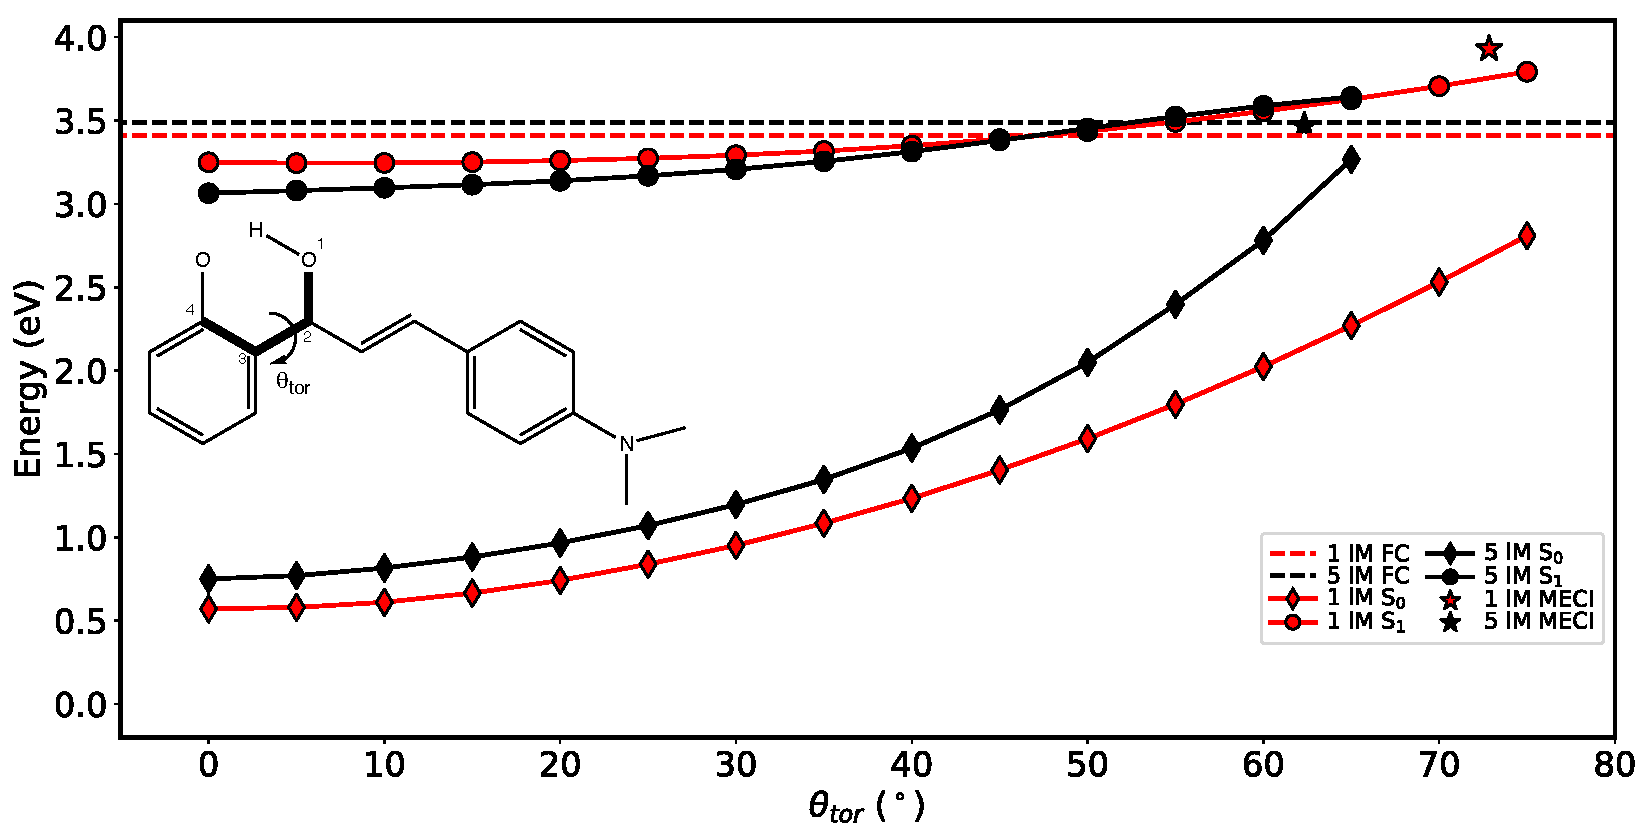
\includegraphics[width=0.8\linewidth]{4IntraInterInteractions/HC_Oniom_Scan.pdf}
  \caption[Relaxed geometry scan in the crystal]{Relaxed geometry scan of the dihedral angle $\theta_{tor}$ calculated at ONIOM($\omega$B97X-D/6-31G(d)):AMBER level of theory for compounds \textbf{1} (red) and \textbf{5} (black) in the \textbf{M15} model. Also plotted are the bright excitation energies (dashed lines) and the MECI energy (stars) for both compounds in the \textbf{M15} model.}
  \label{figure: HC_Oniom_Scan}
\end{figure}

In \textbf{5}, there  exists a double-\Kstar{} state, where both monomers undergo ESIPT. This state is nonemissive in \sone{} (\textit{f}=0.002) lying 0.5 eV above the bright FC state. The localised single proton transfer state in \textbf{5} has emission in the range 2.2-2.3 eV (1.7 eV with CC2). Oscillator strengths, though half the value of the obtained for \textbf{1}, are still significant (0.312 and 0.388). Therefore, while emission from \textbf{1} should be brighter than from \textbf{5}, radiative mechanisms alone cannot explain the negligible quantum yield of \textbf{5}. The structural similarity of the \Estar{} and \Kstar{} minima, namely that the \Estar{} state is planar, means that the pathways no longer compete in the excited state. The bifurcation seen in vacuum is not expected to exist in the solid state, and relaxation to \Kstar{} can follow relaxation in \Estar{}. To maximise the quantum yield, efficient population transfer \Kstar{} is important, since little emissive response will be witnessed from \Estar{} due to the small Stokes shift.

The location of the nearest CI to the \Estar{} and \Kstar{} minima can help understand the balance between radiative and nonradiative decay. In Chapter \ref{chapter:NRdecay}, we saw that in vacuum both pathways lead to energetically accessible conical intersections \textit{via} intramolecular rotation. In the solid, intramolecular rotation in \Estar{} is completely blocked and the \Estar{} CI is accessed instead \textit{via} a stretch of the bridging unsaturated bond. This is associated with an energy cost of upward of 5 eV from the FC \sone{} energy for both crystals. Consequently, molecular aggregation completely blocks the \Estar{} nonradiative decay pathway in both \textbf{1} and \textbf{5}. For \textbf{1}, the \sone/\szero{} MECI associated with the \Kstar{} state lies 0.5-1.0 eV above the \sone{} energy for the FC geometry (Figure \ref{figure: Solid_Mechanism_D7}). For \textbf{5}, the \sone/\szero{} MECI is classically accessible with a barrier of 0.4 eV from the \Kstar{} minimum. While less favourable than in gas phase (barrier 0.2 eV), the system has enough energy to access the conical intersection. Therefore, in compound \textbf{5} the excited state population can decay nonradiatively through the MECI and back to the ground state, whereas in \textbf{1} the population remains in the \Kstar{} state until fluorescence.

\ac{LIIC} between the \Kstar{} minimum and MECI  show the existance of a barrier of 1.4 eV (w.r.t to FC \sone{}) to reach the MECI for \textbf{1} compared to 0.14 for compound \textbf{5}. It is important to state that the LIIC barriers represent an upper bound for barriers on the PES and the true barriers will be smaller, since coordinated relaxation was neglected at each step. However, the barriers here offer further evidence that the MECI of \textbf{1} is inaccessible and \textbf{5} is not. 

\begin{figure}
\centering
  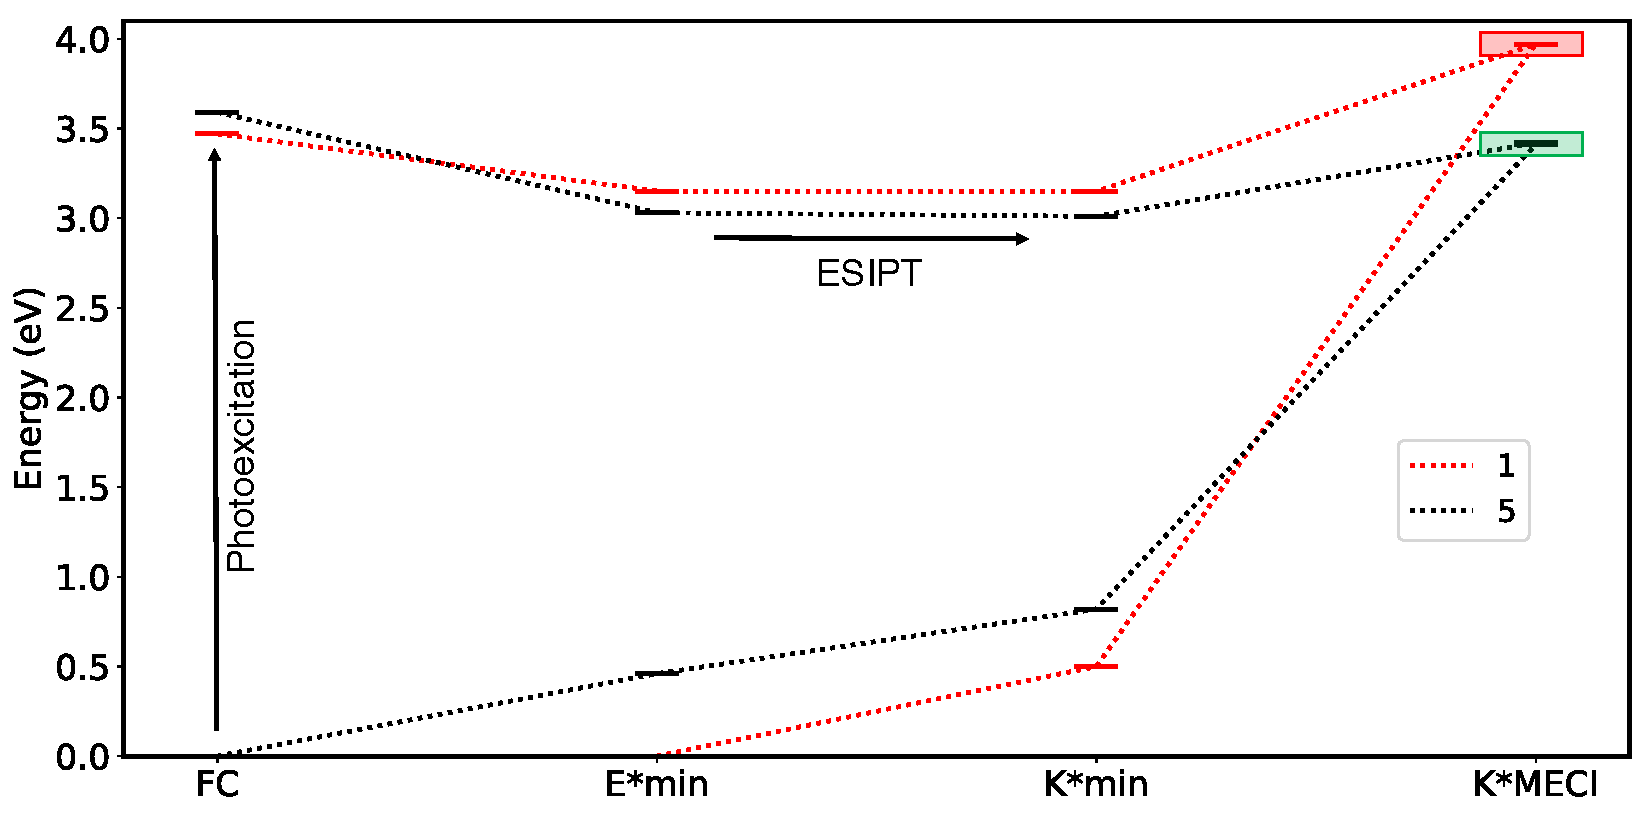
\includegraphics[width=0.8\linewidth]{4IntraInterInteractions/D7.pdf}
  \caption[Decay mechanism in the molecular crystal in \textbf{D7} model]{Energy of the \szero{} and \sone{} states at the  Franck-Condon (FC) point, \Estar{} and \Kstar{} minima, and the MECI of \textbf{1} and \textbf{5} with the \textbf{D7} model with ONIOM($\omega$B7X-D/6-31G(d)):AMBER level of theory. The accessibility is colour coded.}
  \label{figure: Solid_Mechanism_D7}
\end{figure}

\begin{figure}
\centering
  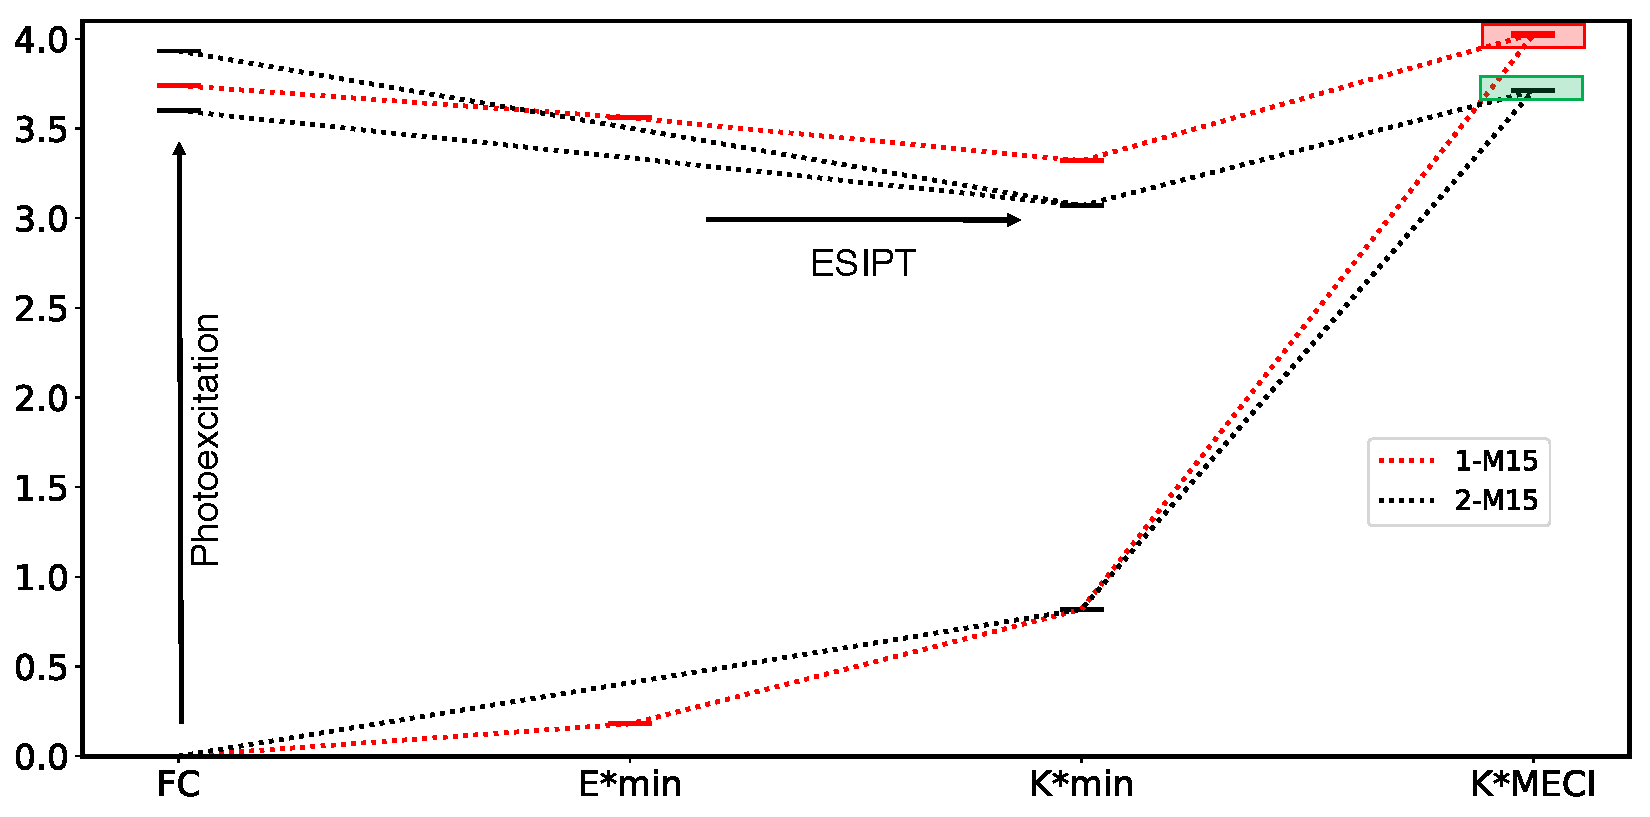
\includegraphics[width=0.8\linewidth]{4IntraInterInteractions/M15.pdf}
    \caption[Decay mechanism in the molecular crystal in \textbf{M15} model]{Energy of the \szero{} and \sone{} states at the  Franck-Condon (FC) point, \Estar{} and \Kstar{} minima, and the MECI of \textbf{1} and \textbf{5} with the \textbf{M15} model with ONIOM($\omega$B7X-D/6-31G(d)):AMBER level of theory. The accessibility is colour coded.}
  \label{figure: Solid_Mechanism_M15}
\end{figure}

\begin{table}
\caption[Relative energies with and without electrostatic embedding in monomer models]{Relative energies for the FC, \Estar{} and \Kstar{} minima, and MECI on the PES for \textbf{1} and \textbf{5} for the \textbf{M7} and \textbf{M15} models, with ME and EE during the optimisation. All values presented in eV relative to the corresponding ground state and are calculated at ONIOM($\omega$B97X-D/6-31G(d)):AMBER level of theory. The oscillator strength \textit{f} is also given.}
\label{table: ONIOM_comparison}
\centering
\begin{tabular}{ccccccccccc} 
\hline
\multicolumn{11}{c}{ Mechanical Embedding (ME) } \\
\hline
&  & \multicolumn{4}{c}{ Compound \textbf{1} } & & \multicolumn{4}{c}{ Compound \textbf{5} } \\
\hline
\multicolumn{2}{c}{} & FC & \Estar{}min & \Kstar{}min & MECI & & FC & \Estar{}min & \Kstar{}min & MECI \\
\hline
\multirow{3}{*}{ \textbf{M15} } & 
S$_{0}$& 0.00 & 0.18 & 0.82 & 4.02 & & 0.00 & - & 0.82 & 3.71 \\ 
& S$_{1}$& 3.74 & 3.56 & 3.32 & 4.03 & & 3.60 & - & 3.07 & 3.71 \\
& \textit{f}& 1.150 & 1.207 & 0.503& - & & 0.749&- &0.475& - \\
\hdashline
\multirow{3}{*}{ \textbf{M7} } & S$_{0}$ & 0.00 & 0.18 & 0.84 & 3.93 & & 0.00 & - & 0.80 & 4.05 \\
& S$_{1}$ & 3.73 & 3.56 & 3.32 & 3.93 & & 3.60 & - & 3.06 & 4.06 \\
& \textit{f}  & 1.511 &1.204 &0.563  & - & & 0.744&- &0.484&-\\

\hline
\multicolumn{11}{c}{ Electrostatic Embedding (EE) } \\
\hline
&  & \multicolumn{4}{c}{ Compound \textbf{1} } & & \multicolumn{4}{c}{ Compound \textbf{5} } \\
\hline
\multicolumn{2}{c}{} & FC & \Estar{}min & \Kstar{}min & MECI & & FC & \Estar{}min & \Kstar{}min & MECI \\
\hline
\multirow{3}{*}{ \textbf{M15} } & S$_{0}$ & 0.00 & 0.10 & 0.59 & 3.93 & & 0.00 & - & 0.84 & 3.47 \\
& S$_{1}$ & 3.41 & 3.31 & 3.25 & 3.93 & & 3.49 & - & 3.04 & 3.48 \\
& \textit{f} & 1.202 & 1.253 &0.928 &- & &0.926&-&0.487&- \\
\hdashline
\multirow{3}{*}{ \textbf{M7} } & S$_{0}$ & 0.00 & 0.08 & 0.48 & 4.04 &  & 0.00 & - & 0.88 & 3.48 \\
& S$_{0}$ & 3.32 & 3.23 & 3.20 & 4.05 & & 3.50 & - & 3.05 & 3.49 \\
& \textit{f} &  0.664 & 1.232 & 1.146 & -& &0.815 &-&0.459&-\\
\hline
\end{tabular}
\end{table}

To further explore the electrostatic effect, the critical points of the \ac{PES} were reoptimised without electrostatic embedding for the monomer models. The energies in comparison to those obtained with electrostatic embedding are given in Table \ref{table: ONIOM_comparison}. Crucially, the accessibility of the MECI depends on its stabilisation with respect to the initially populated excited states. For compound \textbf{1}, the electrostatic potential stabilises the \sone{} state at the FC region but has a smaller effect on the energy of the MECI. Both of these factors decrease the accessibility of the nonradiative channel. A similar effect is seen for both the \textbf{M7} and \textbf{M15} models, suggesting that these are short to medium range effects and are not as a result of long- range Coulombic interactions. For \textbf{5}, the stabilisation of the MECI is larger than for the \sone{} state. Therefore the accessibility of the MECI in \textbf{5} is aided by the short-range electrostatic interactions with the surrounding molecules. 

Moreover, within the mechanical embedding approach, the MECI geometries are similar, but both MECI have energies lying above the photopopulated state for \textbf{5} and below for \textbf{1}. This indicates that steric hindrance in the crystal determines level of distortion of the MECIs, while the Coulombic interactions modulate their total energies. The same conclusions can be drawn from the monomer models, for which the energy levels of \textbf{M15} are shown in Figure \ref{figure: Solid_Mechanism_M15}. As mentioned above, there is  no \Estar{} minimum located for \textbf{5}. As such, it is expected that the short range interactions present in the dimer chromophore restrict torsional relaxation, whilst long range electrostatic interactions, imperfectly included in these models due to the lack of self-consistent polarisation, can help stabilise the excited state, particularly when the geometry of the chromophore most resembles the exterior charge distrubtion, as at absorption.

\begin{figure}
\centering
  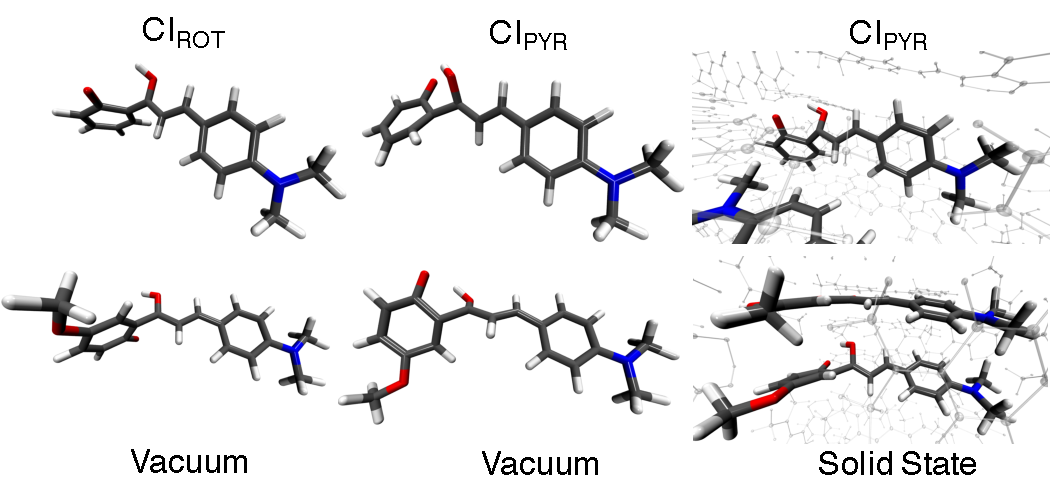
\includegraphics[width=0.8\linewidth]{4IntraInterInteractions/HC_1_5_conicals.pdf}
  \caption[Comparison of vacuum and solid state conical intersections]{Geometry of the \Kstar{} MECI in vacuum (left and center) and in the solid state (right) for \textbf{1} (top) and \textbf{5} (bottom).}
  \label{figure: HC_1_5_conicals}
\end{figure}

The \Kstar{} MECI is accessed \textit{via} a combination of intramolecular rotation (ROT) and carbonyl pyramidalisation (PYR), with a puckering of the deprotonated phenol ring (Figure \ref{figure: HC_1_5_conicals}). In contrast with the most stable conical intersections (CI\textsubscript{ROT}) in vacuum, the MECI structures in the solid state (CI\textsubscript{PYR}) display a significant pyramidalisation of the carbonyl carbon, with a puckering angle of 41\textdegree{}. The puckering angle is defined as the angle between the the (protonated) carbonyl and plane made by the $\alpha$ carbons. The pyramidalisation is at the expense of $\theta_{tor}$, which decreases with respect to the vacuum MECI.  This is caused by the steric restrictions of the surrounding molecules, meaning CI\textsubscript{ROT} can no longer be accessed and the pyramidalised conical intersection becomes the MECI. For \textbf{5}, the \Kstar{} MECI has similar geometric parameters as \textbf{1}, but with a smaller pyramidalisation of the carbonyl group (21\textdegree{}). Interestingly, a similar CI\textsubscript{PYR} conical intersection can be found in vacuum for both compounds, (Figure \ref{figure: HC_1_5_conicals}), with the CI\textsubscript{PYR} lying 0.9 eV above the CI\textsubscript{ROT} for \textbf{1} and 0.6 eV for \textbf{5}. Therefore, the crystal changes the order stability of the conical intersection manifold, stabilising CI\textsubscript{PYR} over CI\textsubscript{ROT} compared to in vacuum. In vacuum, CI\textsubscript{PYR} is energetically accessible in both \textbf{1} and \textbf{5}, lying 0.04 below the \sone{} state for \textbf{1}. For \textbf{5}, CI\textsubscript{PYR} lies 0.33 eV below the initial excitation energy in vacuum. CI\textsubscript{ROT} in vacuum is also accessed at lower rotational distortion and lower energy than the corresponding CI for \textbf{1}. As such, since the accessibility of the conical intersection for \textbf{5} is witnessed in vacuum, the larger stability of the MECI in the solid state compared to \textbf{1} is mainly explained by the electronic effects provided by the methoxy substituent, aided by the electrostatic potential discussed above. As a result, \textbf{5} has enough energy to deactivate through the conical intersection and return to the ground state via the nonradiative pathway, a channel infeasible for compound \textbf{1}. 

\begin{table}
  \centering
  \caption[]{} 
  \label{table: conical_parameters}
  \begin{tabular}{lccccc}
  \hline
  & \multicolumn{2}{c}{Compound \textbf{1}} & \multicolumn{2}{c}{Compound \textbf{5}}\\
  \hline
  & $\theta_{puck}$ & $\theta_{tor}$ & $\theta_{puck}$ & $\theta_{tor}$ \\
  \hline
  Vacuum CI\textsubscript{ROT} & 8\textdegree{} & 89\textdegree{} & 5\textdegree{} & 90\textdegree{}\\
  Vacuum CI\textsubscript{PYR} & 65\textdegree{} & 36\textdegree{} & 62\textdegree{} & 27\textdegree{}\\
  Solid (\textbf{sD}) CI\textsubscript{ROT} & 65\textdegree{} & 41\textdegree{} & 67\textdegree{}&21\textdegree{}\\
  \hline
  \end{tabular}
\end{table}

\section{Summary and Conclusions}\label{section: Inter_conclusions}

In summary, the analysis of two materials with contrasting emissive properties illustrates how the balance of intermolecular and intramolecular factors can control the radiative and nonradiative mechanisms underlying their light response. The relaxation mechanisms for \textbf{1} and \textbf{5} shown in Figures \ref{figure: HC_1_Density_Mechanism} and \ref{figure: HC_5_Density_Mechanism}. After initial photoabsorption the excited state is delocalised in the enol form, where $\pi$-$\pi$ interactions in \textbf{5} increase the excitonic coupling, which plays a role at the Franck-Condon state where absorption is delocalised. In the next chapter, the delocalisation of the exciton in the enol channel shall be scrutinised. The systems relax in \Estar{}, where a minimum exists on the PES and emission with very small Stokes shift is possible, but self-absorption would most likely be witnessed. Nonradiative decay through a conical intersection in the enol channel is unlikely due to its high energy. 

Alternatively, localisation allows ESIPT, followed by relaxation. For \textbf{1}, the nearest MECI in the \Kstar{} channel is classically inaccessible and so fluorescence is witnessed. For \textbf{5}, the MECI is lower in energy, due to the difference in electronic density distribution in \sone{} on account of the methoxy group, and the wavepacket can funnel nonradiatively to \szero{}. For the \Kstar{} channel, the crystal changes the relative energy of two conical intersections present in gas phase, stabilising a structure where the carbonyl group pyramidalises. The calculations show that either nonradiative delocalised transport processes (\Estar{} channel) or localised deactivation through the ESIPT (\Kstar{} channel) are more likely in \textbf{5} than in \textbf{1}. The interplay of all discussed factors results in an enhance emissive response of \textbf{1} and no fluorescence in \textbf{5} in the solid state. 

\begin{figure}
  \centering
  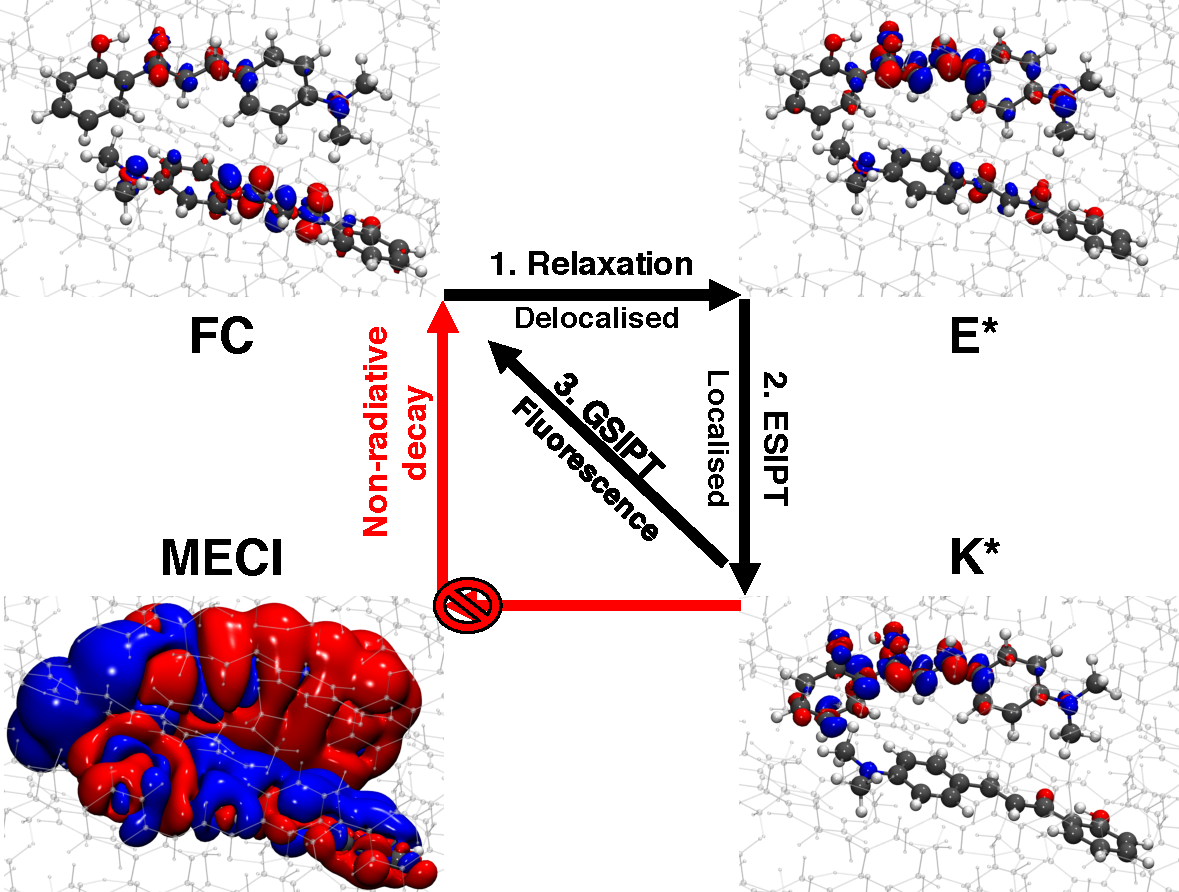
\includegraphics[width=0.8\linewidth]{4IntraInterInteractions/HC_1_Density_Mechanism.pdf}
  \caption[Radiative decay in \textbf{HC1}]{The mechanism for nonradiative decay in compound \textbf{2}. Also shown are \sone-\szero{} electron density differences (red: \sone{}, blue: \szero{}).}
  \label{figure: HC_1_Density_Mechanism}
\end{figure}

\begin{figure}
  \centering
  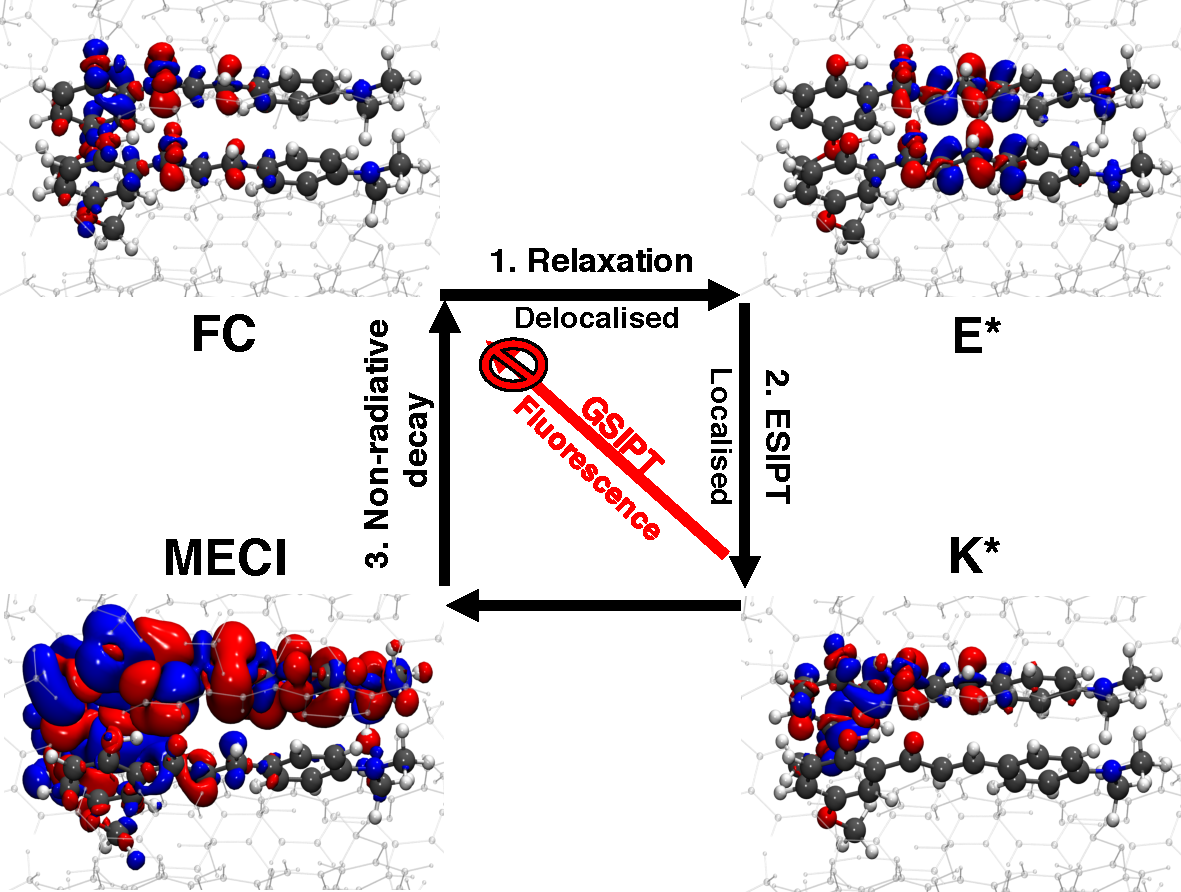
\includegraphics[width=0.8\linewidth]{4IntraInterInteractions/HC_5_Density_Mechanism.pdf}
  \caption[Nonradiative decay in \textbf{HC5}]{The mechanism for nonradiative decay in compound \textbf{5}. Also shown are \sone-\szero{} electron density differences (red: \sone{}, blue: \szero{}).}
  \label{figure: HC_5_Density_Mechanism}
\end{figure}

From these results, some design principles can be proposed for more efficient solid-state emitters. As strong electrostatic interactions aid the deactivation through nonradiative pathways, it is clear why many of the reported AIE fluorophores are nonpolar. For the ESPIT chromophores, stabilising \Estar{} over \Kstar{} minima could be favourable because the \Estar{} nonradiative pathway through a conical intersection is hampered in the solid state. For this, the nature of the \Estar{} state must be altered to induce a larger Stokes shift. Alternatively, if the \Estar{} state is made more unstable by increasing the lability of the transferring proton, the population transfer to the \Kstar{} channel will increase. To maximise returns, access to the pyramidal \Kstar{} MECI can be further hindered by imposing geometrical restrictions, such as introducing fused rings to the molecular structure. Other studies in ESIPT systems have shown that torsional restraint can also be achieved by coordination to metals.\cite{Karsili2016} For the \Kstar{} channel, efficient localisation of excited state to one monomer, bias for \Kstar{} over \Estar{} decay and an energetically inaccessible conical intersection are all highly desirable. Indeed path agnosticity for compound \textbf{1}, which is evenly distributed for \Estar{} and \Kstar{}, may prevent efficient transfer to the emissive \Kstar{} state. This is remedied in \textbf{5} by the bias for ESIPT but the low-lying MECI prevents fluorescence. The design of a chromophore to combine the \Kstar{} bias of \textbf{5} with the stability of \textbf{1} would surely be a promising candidate for a highly efficient fluorophore.  In the next chapter a new class of AIE system based on the \textbf{HC} family shall be introduced and investigated, building on the conclusions of Chapters \ref{chapter:NRdecay} and \ref{chapter: Inter} for fluorophore design. 